In previous sections, we showed that distance functions alone could help to identify low impact edits that lead to test cases that can be updated with little effort. Moreover, the case study in Section \ref{sec:case} showed that this strategy could reduce test case discard by 9.53\%. Although very promising, we believe those results could be improved, especially regarding the classification of \textit{high impact }edits. In this sense, we propose a complementary strategy that combines distance values and machine learning.

%Machine Learning is a branch of Artificial Intelligence based on the idea that systems can learn from data, identify patterns, and make decisions with minimal human intervention \cite{michie1994machine}. By providing ways for building data-driven models, machine learning can produce accurate results and analysis \cite{zhang2003machine}. The use of machine learning in software engineering has grown in the past years. For instance, machine learning methods have been used for: estimating development effort \cite{srinivasan1995machine,baskeles2007software}, predicting a software fault-proneness \cite{gondra2008applying}, fault prediction \cite{shepperd2014researcher}, and improving code quality \cite{malhotra2012fault}.

To apply machine learning and avoid test case discard, we used Keras \citep{gulli2017deep}. Keras is a high-level Python neural networks API that runs on top of TensorFlow \citep{abadi2016tensorflow}. It focuses on efficiency and productivity; therefore, it allows easy and fast prototyping. Moreover, it has a stronger adoption in both the industry and the research community \citep{geron2019hands}.

Keras provides two types of models \textit{Sequential}, and \textit{Model with the functional API}. We opted to use a Sequential model due to its easy configuration and effective results.
%being easier to use, to code, and to build models. Functional Models can get cumbersome as not necessarily one layer comes after the other. Moreover, we intend to do an exploratory study, varying the number of layers, knots, and functions to find the best configuration and optimal models. This task is made easier using sequential models, although it does not have the flexibility of functional models. 
A sequential model is composed of a linear stack of layers. Each layer contains a series of nodes and performs calculations. A node is activated only when a certain threshold is achieved. In the context of our model, we used the REctified Linear Units (ReLU) and Softmax functions. Both are known to be a good fit for classification problems \citep{agarap2018deep}. Dense layer nodes are connected to all nodes from the next layer, while Dropout layer nodes are more selective. 

Our model classifies whether two versions of a given test case step refer to a \textit{low} or \textit{high impact} edit. Although techniques such as Word2Vec \citep{rong2014word2vec} could be used to transform step descriptions to numeric vectors, due to previous promising results (Sections \ref{sec:es} and \ref{sec:case}), we opted to use a classification based on a combination of different distance values. Therefore, to be able to use the model, we first pre-process the input (versions of a test step), run the ten functions (Hamming \citep{hamming1950error}, LCS \citep{han2007efficient:LCS}, Cosine \citep{huang2008similaritycosine}, Jaro \citep{de1mahalanobis:jaro}, Jaro-Winkler \citep{de1mahalanobis:jaro}, Jaccard \citep{Lu2013SimilaridadeJaccard}, Ngram \citep{Kondrak2005ngram}, Levenshtein \citep{Levenshtein_SPD66}, OSA \citep{Damerau:1964}, and Sorensen Dice \citep{sorensen1948method}), and collect their distance values. Those values are then provided to our model that starts with a Dense layer, followed by four hidden layers, and returns as output a size two probability array $O$. $O$'s first position refers to the found probability of a given edit be classified as\textit{ high impact}, while the second refers to the probability for a \textit{low impact} edition. The highest of those two values will be the final classification of our model. 

Suppose two versions of the test step \textit{s} (\textit{s} and \textit{s'}). First, our strategy runs the ten distance functions considering the pair \textit{(s; s')} and generates its input model set (e.g., $I = {0.67; 0.87; 0.45; 0.78; 0.34; 0.6; 0.5; 0.32; 0.7; 0.9}$). This set is then provided to our model that generates the output array (e.g., $O = [0.5; 0.9]$). For this example, $O$ indicates that the edits that transformed \textit{s} to \textit{s'} are \textit{high impact}, with 50\% chances, and \textit{low impact}, with 90\% chances. Therefore, our final classification is that the edits were \textit{low impact} edit. 

% Figure \ref{fig:overview2} summarizes our classification strategy.

% \begin{figure}[h]
% \centering
% 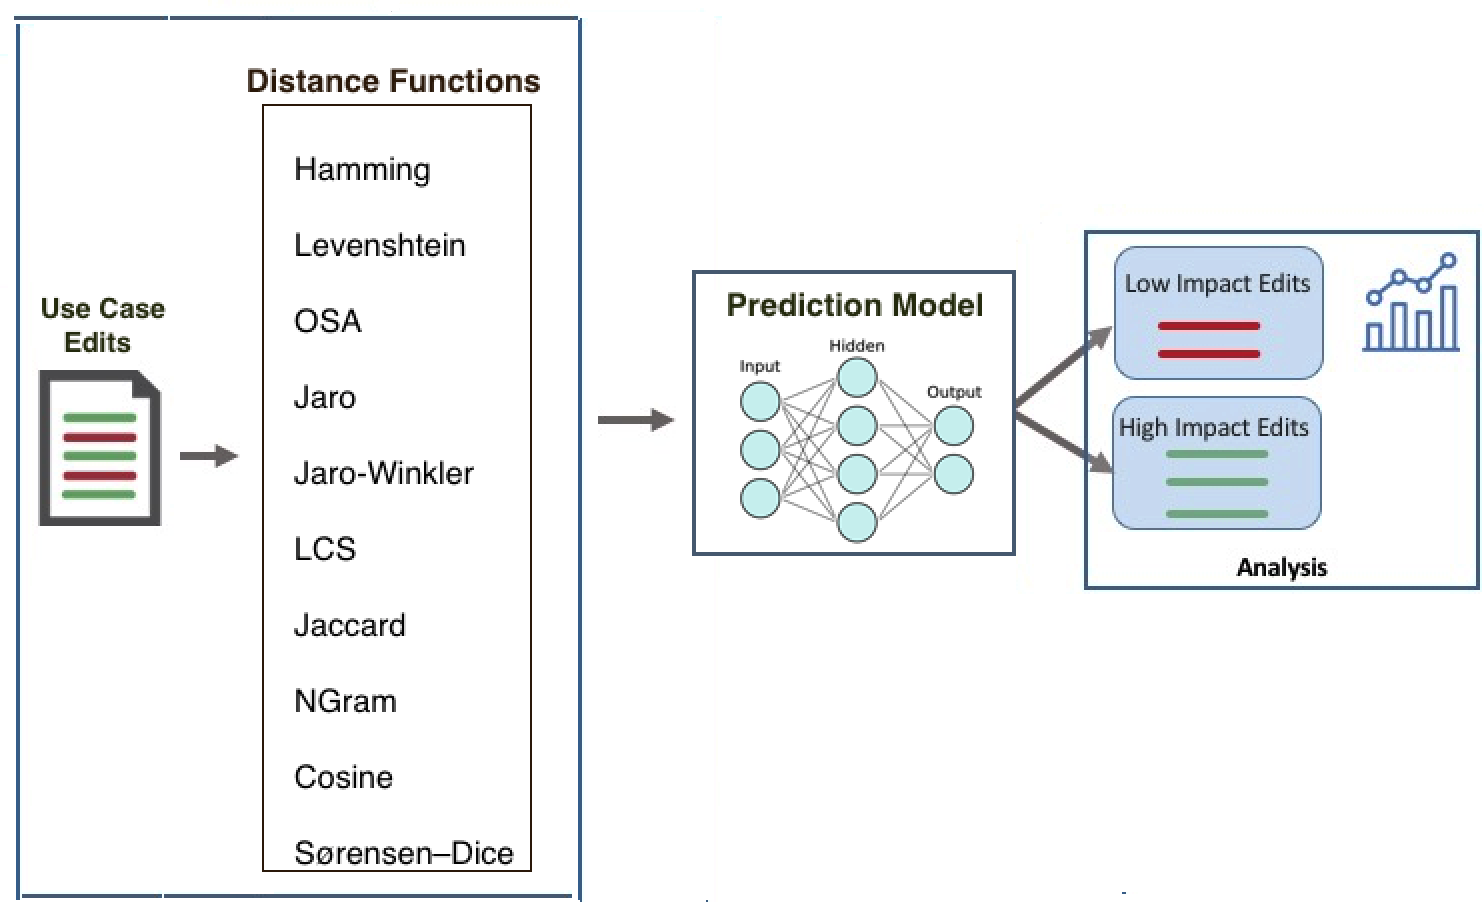
\includegraphics[height=2.3in,width=3.3in]{figs/overview2.png}
% \caption{Overview of the combined strategy for a single subject.}
% \label{fig:overview2}
% \end{figure}

For training, we created a dataset with 78 instances of edits randomly collected from both SAFF and BZC projects. To avoid possible bias, we worked with a balanced training dataset (50\% \textit{low impact} and 50\% \textit{high impact} edits). Moreover, we reused the manual classification discussed in Sections \ref{sec:emp} and \ref{sec:es} as reference answers for the model. In a Notebook Intel Core i3 with 4GB of RAM, the training phase was performed in less than 10 minutes.


\subsection{Model Evaluation}

Similar to the investigation described in Sections \ref{sec:es} and \ref{sec:case}, we proceeded an investigation to validate whether the strategy that combines machine learning with distance values is effective and promotes the reduction of test case discard. For that, we set the following research questions:
\begin{itemize}
\item \textbf{RQ7}: Can the combination of machine learning and distance values improve the classification of edits' impact in use case documents?

\item \textbf{RQ8}: Can the combination of machine learning and distance values reduce the discard of MBT tests?

%\item \textbf{RQ7}: Can the combination of machine learning and distance values be used to classify the impact of edits in use case documents?

%\item \textbf{RQ8}: Can the combination of machine learning and distance values be used for reducing the discard of MBT tests?
\end{itemize}

To answer RQ7, and evaluate our model, we first ran it against two data sets: (i) the model edits combined of the SAFF and BZC projects (Table \ref{tab:useCases}); and (ii) the model edits collected from the TCOM project (Table \ref{tab:useCasesEvaluation}). While the first provides a more comprehensive set, the second allows us to test the model in a whole new scenario. It is important to highlight that both data sets contain only real model edits performed by the teams. Moreover, they contains both \textit{low} and \textit{high impact} edits. Again, we reused our manual classification to validate the model's output. Table \ref{tab:tcomEval} presents the results of this evaluation. As we can see, our strategy performed well for predicting the edits impact, especially for TCOM, it provided an accuracy of 95\%. These results give us evidence of our model efficiency.
\\ 
\\
\noindent
\vspace{2mm} %5mm vertical space
\fbox{\begin{minipage}{23em}
\textbf{RQ7: Can the combination of machine learning and distance values improve the classification of edits' impact in use case documents?}
Our strategy was able to classify edits with accuracy above 80\%, an improvement of 7\% when compared to the classification using only distance functions. This result reflects its efficiency.
%\textbf{RQ7: Can the combination of machine learning and distance values be used to classify the impact of edits in use case documents?}
%Our strategy was able to classify edits with accuracy above 80\%, which reflects its efficiency.
\end{minipage}}
\vspace{2mm}

\begin{table}[]
\centering
\caption{Results of our model evaluation using TCOM's dataset.}
\label{tab:tcomEval}
\begin{tabular}{|l|l|l|l|}
\hline
     & \textbf{Precision} & \textbf{Recall} & \textbf{Accuracy} \\ \hline
\textbf{SAFF+BZC} &     81\%      &      97\%    &     80\%         \\  \hline
\textbf{TCOM} &     94\%      &      99\%    &     95\%         \\  \hline
\end{tabular}
\end{table}

To answer RQ8, we considered TCOM’s MBT test cases generated from its CLARET files. We reused the manual classification from Section \ref{sec:case}, and ran our strategy to automatic reclassify the 724 obsolete test cases among \textit{low impacted} – test cases that include unchanged steps and updated steps classified by our strategy as ``low impact''; \textit{highly impacted} – test cases that include unchanged steps and ``high impact'' steps; and \textit{mixed}, test cases that include at least one ``high impact'' step and at least one ``low impact'' step.

% functions
%         LP    HP    MP    
% LA    69    3    37    109
% HA    4    37    155    196
% MA     21    27    371    419
%         94    67    563    724

% model
%       LP    HP    MP    
% LA    75    4    30    109
% HA    12    169    15    196
% MA     6    157    256    419
%       93    330    301    724

From the 109 actual \textit{low impacted} test cases, our strategy was able to detect 75 (69\%), an increase of 6\% when compared to the classification using a single distance function. Those would be test cases that should be easily revised to avoid discarding as model changes were minimal (Figure \ref{tab:li_tc}). Table \ref{tab:conf_mat2} presents the confusion matrix for our model classification. Out of the 724 obsolete test cases (according to Oliveira et al.’s classification \citep{de2016full}), our model would help a tester to automatically save 10.4\% from discarding. 

As we can see, overall, our classification was 69\% effective, an increase of 3\% when compared to the classification using a single distance function (Table \ref{tab:conf_mat}). Although this improvement may be low, it is important to remember that those would be the actual test that would be saved from a wrong discard.

On the other hand, we can see a great improvement in the \textit{high impact} classification (from 19\% to 86\%). This data indicates that different from the strategy using a single distance function, our model can be a great help to automatically identify both reusable and in fact obsolete test cases. On the other hand, the classification for \textit{mixed} test cases performed worse (from 88\% to 61\%). However, we believed that mixed test cases are the ones that require a manual inspection to check whether it is worth updating for reusing or should be discarded. 

It is important to highlight that our combined strategy was able to improve the performance rates for the most important classifications (\textit{low} and \textit{high impacted}), which are related to major practical decisions (to discard or not a test case). Moreover, when wrongly classifying a test case, our model often sets it as \textit{mixed}, which we recommend a manual inspection. Therefore, our automatic classification tends to be accurate and not misleading. 

Finally, we can answer RQ8 by saying that the combined strategy was, in fact, effective for reducing the discard of MBT tests. The rate of saved tests was 10.4\%. Moreover, it improved, when compared to the strategy using a single distance function, the detection rate by 6\% for \textit{low impacted} test cases, and by 67\% for \textit{high impact} ones. 
\\
\\
\noindent
\vspace{2mm} %5mm vertical space
\fbox{\begin{minipage}{23em}
\textbf{RQ8: Can the combination of machine learning and distance values reduce the discard of MBT tests?}
%\textbf{RQ8: Can the combination of machine learning and distance values be used for reducing the discard of MBT tests?}
Our combined strategy helped us to reduce the discard of test cases by 10.4\%, an increase of 0.9\%. However, it correctly identifies test cases that should in fact be discarded.
\end{minipage}}
\vspace{2mm}




